% !TEX root = ../lectures_olympics.tex

\chapter{相对论}

\section{相对论的发现}
 \begin{wrapfigure}{o}{4cm}
 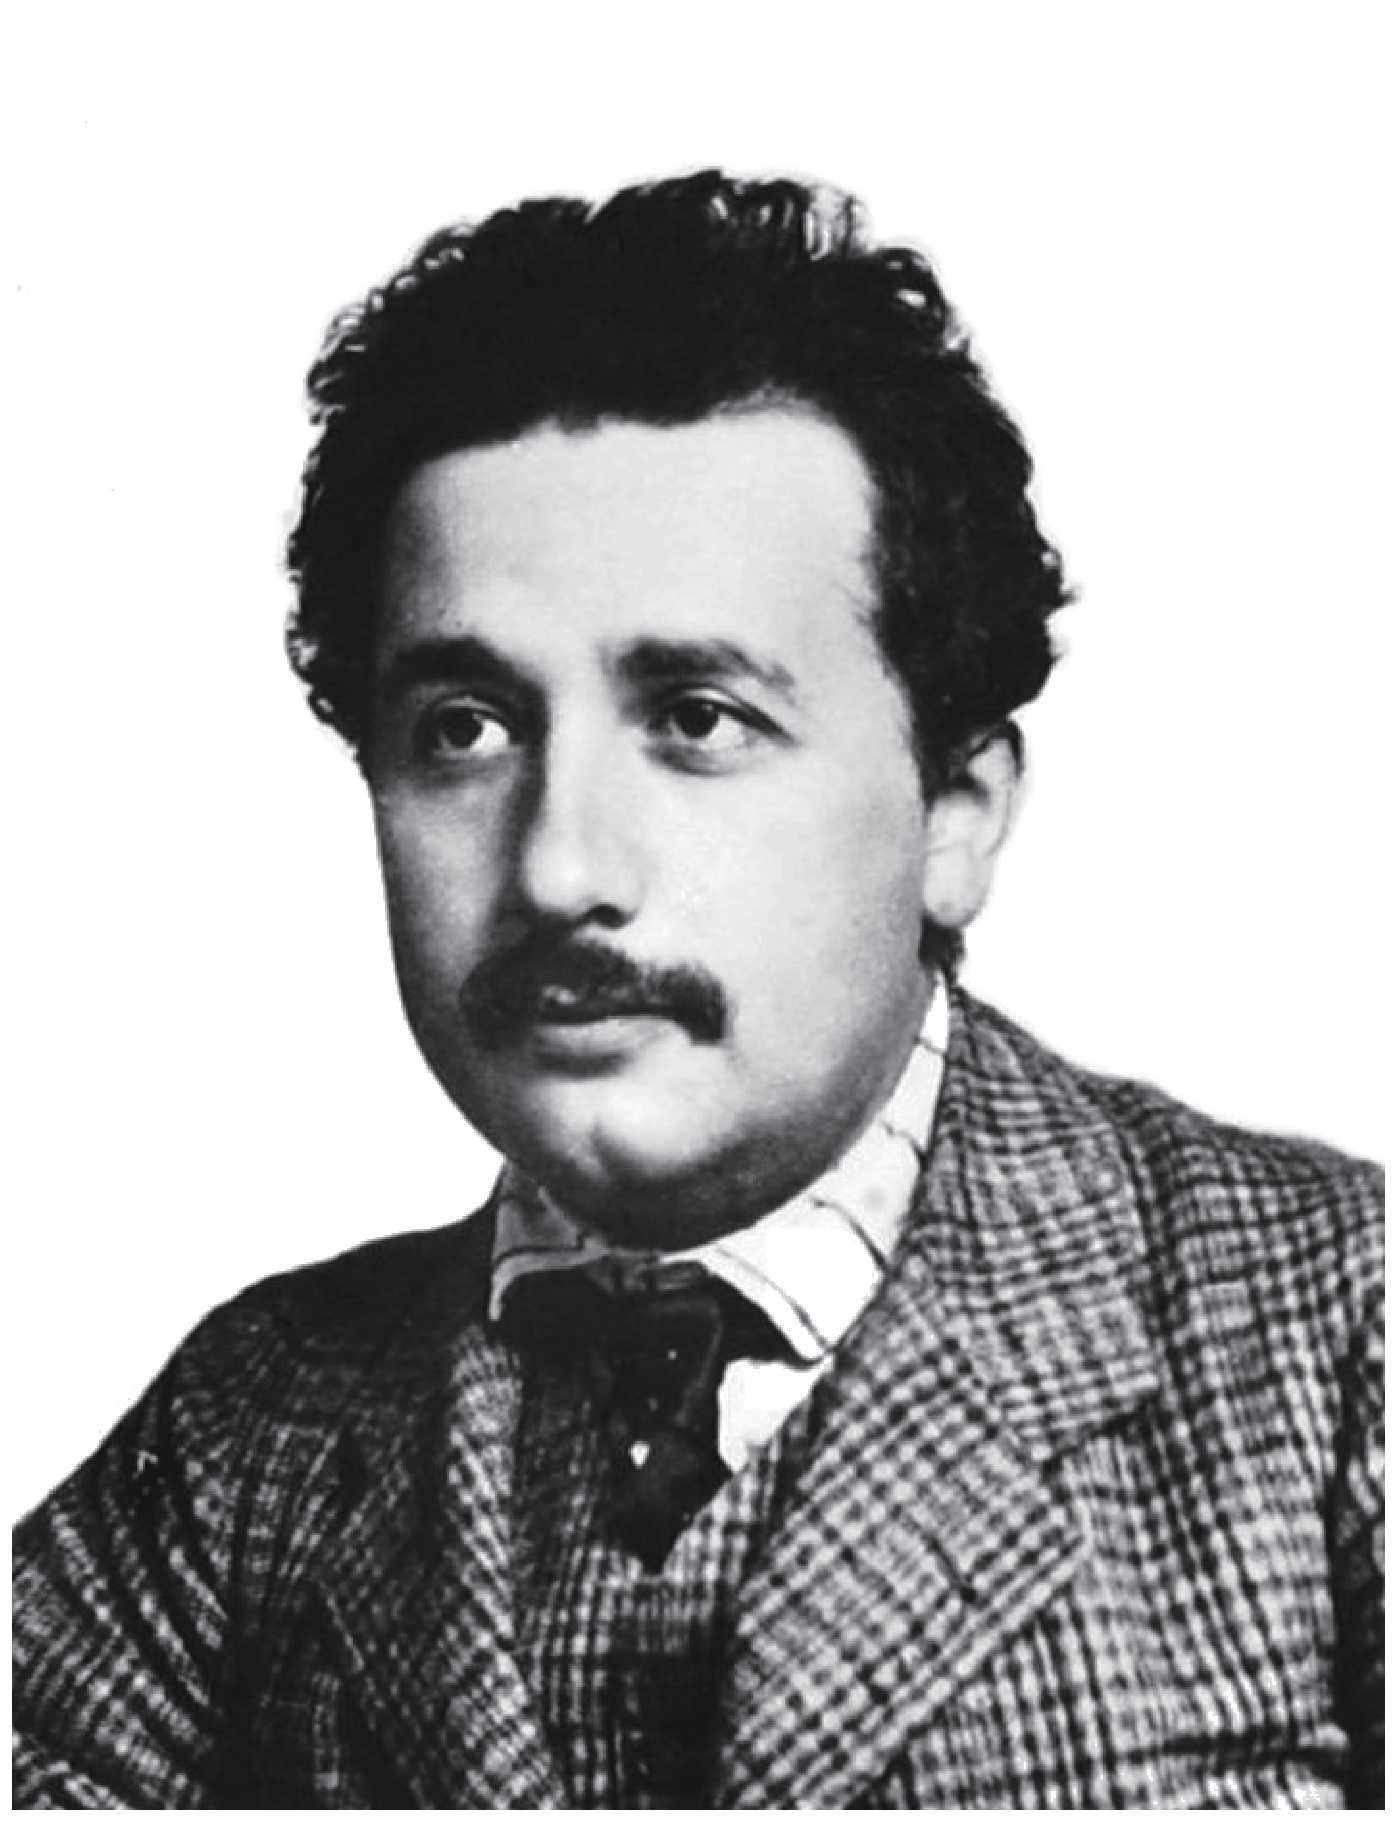
\includegraphics[width=4cm]{images/relativity-4.pdf} 
 \caption{爱因斯坦}
 \end{wrapfigure}
在前面我们已经学过了电磁学的主要内容,其中最引人注目的现象就是电磁波。
由于磁场的变化引起的涡旋电场和由于电场变化产生的位移电流使得电磁振荡不断地向远处传递而形成了电磁波,它的出现极大地改变了世界的面貌。
电磁波的发现给了当时的人们一个惊喜,电磁辐射传递的速度,也就是电磁波的波速是由来自于静电学和静磁学的两个基本参数$\epsilon_0$和$\mu_0$所决定:
\begin{equation}
c=\frac{1}{\sqrt{\varepsilon_0\mu_0}},
\end{equation}
这个速度与当时已知的光速相吻合,这最终使电磁学的创始人麦克斯韦({\it J. C. Maxwell})相信光就是电磁波,不同颜色光对应于不同波长的电磁波。
这一假设很快被实验所证实。

但是电磁学与牛顿力学的伽利略时空观有一个深刻的矛盾,它与光速的性质密切相关。
考虑地面上一列以速度$v$匀速行驶的火车,假设车头有一个光源,向着火车前进的方向发出一束光。
毫无疑问相对于火车这束光的速必然是光速$c$,但是相对于地面这束光的速度又是多少呢?
根据我们学过的速度叠加的法则,很自然地得出这束光相对于地面的速度是光速和火车速度的和$v+c$。
但是相对于地面,由车头光源发出的光也是由电场、磁场相互感应而形成的电磁波,而且实验表明真空的介电常数$\varepsilon_0$和真空磁导率$\mu_0$与参考系的运动状态并没有什么关系,这也意味着光,也就是电磁波相对于地面的速度理应也是$c$。
如何调合这一对矛盾在当时是不清楚的。

可以设想很多这样的实验,相对于地面光源可以以任意的速度运动,坚持前面的逻辑我们应当观察到各种各样的光速。
在物理上解决矛盾的办法自然是通过实验来观测自然界到底是怎么样的。
鉴于当时人造物体的速度相对于光速都太小,而且测量一个运动光源发出光的光速也很困难,所以为了测量光速的变化人们采取了另外的方法。
自然界中当时能够被利用的最快速度是地球围绕太阳的公转,为止迈克尔逊({\it A. A. Michelson})和莫雷({\it E. W. Morley})设计了著名的干涉仪。


\begin{figure}[htb]
\centering
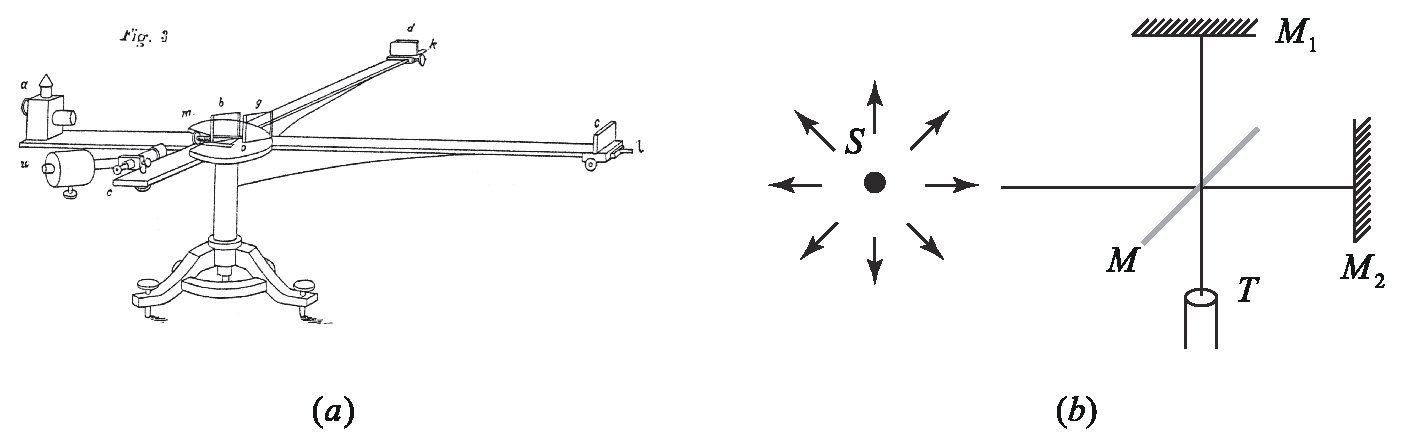
\includegraphics[width=0.9\textwidth]{images/relativity-5.pdf}
\caption{迈克尔逊-莫雷实验:(a)装置(b)原理}
\label{fig: relativity-5}
\end{figure}

迈克尔逊和莫雷于 1887 年利用灵敏的干涉仪,企图用光学方法测定地球的绝对运动。
实验时先使干涉仪的一臂与地球的运动方向平行,另一臂与地球的运动方向垂直。
按照经典的理论,在运动的系统中,光速应该各向不等,因而可看到干涉条纹。
再使整个仪器转过$90^\circ$,就应该发现条纹的移动,由条纹移动的总数,就可算出地球相对
于以太运动的速度$v$。
{\heiti 迈克尔孙—莫雷实验}(Michelson-Morley experiment)的装置如图所示,使一束由光源$ S $射来的平行光到达对光线倾斜$45^\circ$角的半镀银镜面$ M $上,被分成两束互相垂直的相干光。
其中透射部分沿$MM_2 $方向前进,被镜$ M_2 $反射回来到$ M $上, 再部分地反射后沿$ MT $进行;反射部分沿$ MM_1 $方行进行,被镜反射回来后再到达$M $上,光线部分透过,也沿$ MT $进行。
这两束光在$ MT $方向上互相干涉,而在$ T $处观察或摄影,由于$ MM_2$臂沿着地球运动方向,臂$MM_1$垂直于地球运动方向,若$MM_2= MM_1=L$,地球的运动速度为$ v$,则两束光回到$ M $点的时间差为
\[
\Delta t = \frac{L}{c}\left(  \frac{v}{c}\right)^2.
\]
当仪器绕竖直轴旋转$ 90^\circ $角,使$MM_1$变为沿地球运动方向,$MM_2$垂直于地球运动方向, 则两束光到达$ M $的时差为
\[
\Delta t' = -\frac{L}{c}\left(  \frac{v}{c}\right)^2.
\]
我们知道,当时间差的改变量是光波的一个周期$ T_1 $时,就引起一条干涉条纹的移动,所以
当仪器转动$90^\circ $后,在望远镜$ T $处看到的干涉条纹移动的总数为
\begin{equation}
\Delta N = \frac{ \Delta t- \Delta t'}{T_1} = \frac{2L}{ 	\lambda}\cdot \frac{v^2}{c^2},
\end{equation}
式中$ \lambda$是波长,当$ L=11 $米,$ v = 3\pow{4}\unit{m/s}$ ,$ c = 3\pow{8}\unit{m/s}$,所用光波的波长$ \lambda = 5.9\pow{-7}~\text{m}$,根据上式算出的$ \Delta N  \approx 0.4$。
这相当于在仪器旋转前为明条纹,旋转以后几乎变为暗条纹。
但是他们在实验中测得$ \Delta N \approx \frac{1}{100}$,而且无论是在白天、夜晚以及一年中的所有季节进行实验,始终得到否定的结果。
就是说光学的方法亦测不出所在参考系(地球)的运动状态,而结果是我们没有观测到光速与$c$的任何偏离。

一边是刚刚建立并取得极大成功的电磁学,一边是经历了200多年实践检验的牛顿力学,它们之间的矛盾在当时令人们不知所措。
而此时历史选择了{\heiti 爱因斯坦}({\it A. Einstein}),他认为电磁学定律在所有的惯性参考系当中都成立,最直接的推论就是光速在所有的惯性参考系中都有相同的数值,与光源的运动状态以及光运动的方向无关,这就是{\heiti 光速不变假说}(one-way speed of light)。
更进一步,不仅是电磁学,所有的物理定理在所有的惯性参考系都成立,并且具有相同的形式,这就是从牛顿以来人们一直坚持的{\heiti 相对性原理}(principle of relativity)。在这两条原理的基础上,爱因斯坦建立了著名的{\heiti 狭义相对论}(special relativity)。




\section{新的时空理论}
为了同时满足相对性原理和光速不变,就必须改变数千年来我们对空间、时间的观念。

在讨论时空的性质之前有必要首先明确一个物理概念:{\heiti 事件}(event)。
一个事件实际上就是发生的一件事,而且这件事有着明确的判别标准。
例如,发生了一个爆炸就可以称为一个事件,一个飞行着的粒子突然解体(衰变)也是一个事件,一个光源发出的光到达一个给定的探测器也是一个事件。
一个事件的发生是客观的,而且是绝对的,并不依赖于我们观察和描写它的方式。例如光源发出的光从不同角度,以不同相对速度看其角分布都是不同的,但它们都是同一个事件,具有相同的物理内容,只是数学描写的数值不相同而已。

最后,物理学上抽象的事件模型要求其发生在某一个时空点上。类比于质点模型的抽象过程,日常生活中的``事件''往往发生于一小段时间间隔内,而且具有一定大小的空间广延性。这样的时间,空间区域大小如果相对于我们研究的问题的特征时空尺寸足够地小,就可以抽象为一个个事件。而我们研究的物理过程,则是由空间上连绵展开,时间上相继进行的无数个事件的和。物理上抽象出来的事件由两组物理量描述:一是事件发生的{\heiti 时空坐标}(spacetime coordinates);二是描述事件本身特征的物理量,它可以是标量(如某次爆炸放出的能量),矢量(如粒子运动的瞬时速度)或是更复杂的情况。


\begin{figure}[htb]
\centering
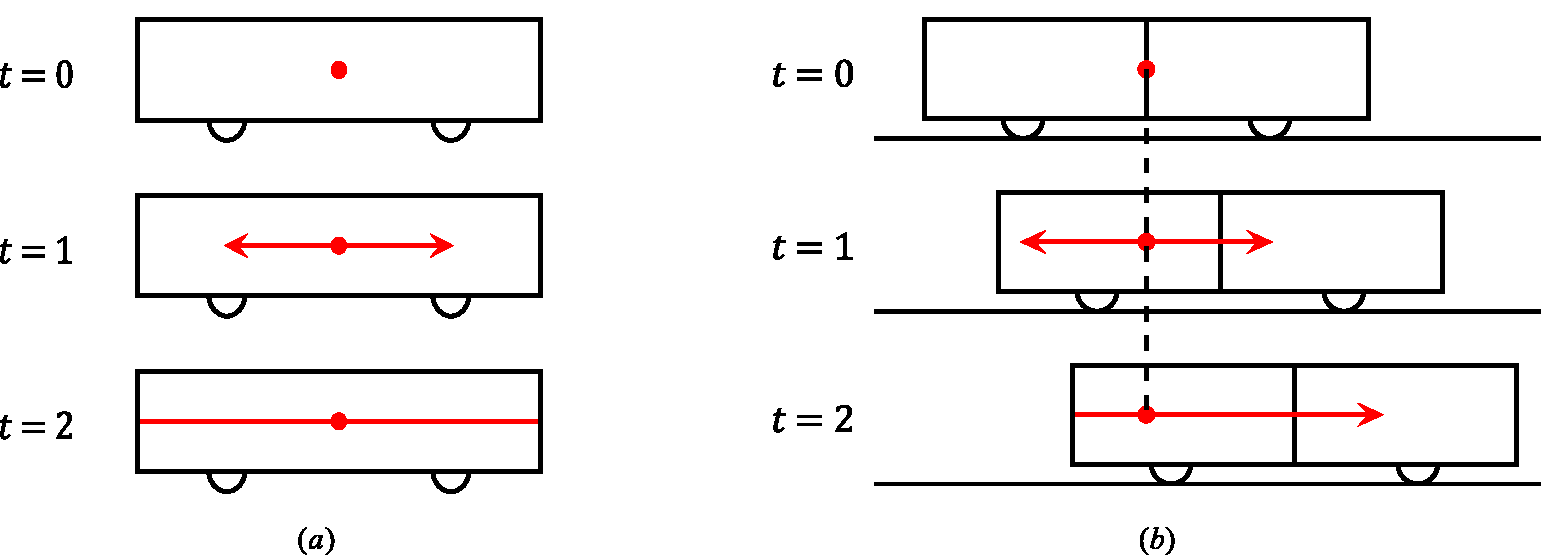
\includegraphics[width=0.7\textwidth]{images/relativity-6.pdf}
\caption{火车中部发出的光到达车头和车尾的时间}
\label{fig: relativity-6}
\end{figure}

考虑一列长度为$2L$,以速度$v$匀速直线行驶的列车,在列车正中部有一个光源。
这个光源发出了光线,当然这是一个明确的事件。
在相对于火车静止的观察者看来,光向着四面八方传播,因为它是一个惯性参考系,根据光速不变原理,它所测到的光速是一个给定值,这样他会得到这样的结论:光会同时被位于车头和车尾的探测器所接收。
对于另一个与地面相对静止的观察者来说,在他看来光速也是一个给定值。
由于在他看来火车,当然包括车头和车尾却是以$v$做匀速运动,无论它测到火车的长度是多少,车尾必然比车头先接收到火车中部发出的光线。
假设在他看来火车的长度为$2L'$,那么光线到达车头和车尾的时刻分别为
\begin{equation}
t_h=\frac{L'}{c-v},\qquad t_b=\frac{L'}{c+v}
\end{equation}
很容易看到$t_h>t_b$。
对于一个观测者来说同时发生的事件对于另一个观测者则是一前一后发生,坚持相对论的两条基本假设的第一个重要结果就是{\heiti 同时的相对性}(relativity of simultaneity),而在牛顿力学框架下对于同时发生的两个事件不同的惯性参考系必定会给出一致的答案。


\begin{figure}[htb]
\centering
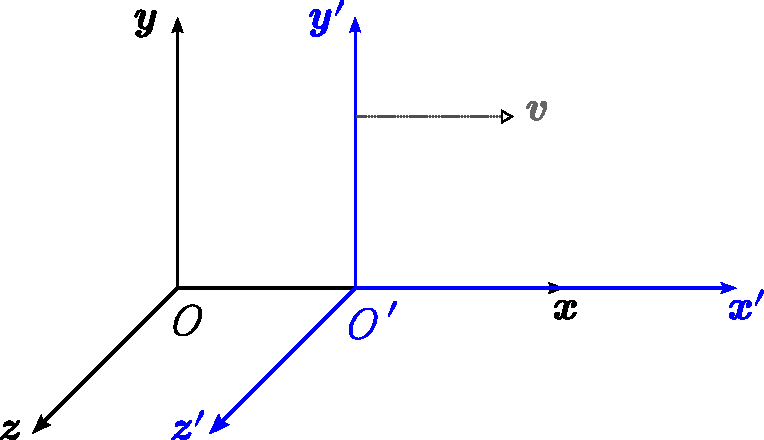
\includegraphics[width=0.5\textwidth]{images/relativity-3}
\caption{两个相对运动参考系}
\label{fig:relativity-3}
\end{figure}


每个惯性参考系都有权利选择它自己的空间和时间,对于同一个事件他们会记录到各自不同的空间位置和发生时刻。
不同的参考系当中对于同一个事件所记录到的空间位置和时间则由两个参考系之间的相对运动产生关联,这样的关联被称做{\heiti 洛伦兹变换}(lorentz transformation)。
假设我们有两个参考系$S$和$S'$,它们用各自的时空坐标给出事件的描述。
在$S$系中建立直角坐标系$(x,y,z)$,原点为$O$,它所用的时间由$t$给出。
同样$S'$系也有相对于它静止原点为$O'$的直角坐标系$(x',y',z')$,而它记录事件所用的时间为$t'$。
假设$S'$系所使用的坐标轴与$S$系平行,并且$S'$的$x'$轴以速度$v$沿着$S$系的$x$轴正方向匀速运动,而在某一时刻它们的原点$O$和$O'$恰好重合,两个惯性参考系原点重合的事件在两个参考系当中发生的时间都是0。
这样任何一个事件被两个参考系所记录到的时空坐标之间就由{\heiti 洛伦兹变换}(Lorentz transformation)相联系:
\begin{eqnarray}
x'&=&\frac{x-vt}{\sqrt{1-\frac{v^2}{c^2}}}\label{eqn: x的Lorentz变换}\\
y'&=&y\\
z'&=&z\\
t'&=&\frac{t-\frac{v}{c^2}x}{\sqrt{1-\frac{v^2}{c^2}}}\label{eqn: t的Lorentz变换}
\end{eqnarray}


%%%%%%%%%%%%%%%%%%%%%%%%%%%%%%%%%%
\begin{example}
有两个相对运动的参考系$S$、$S'$,$S'$沿着$x$轴正方向以速度$v=0.8c$运动,在$t = t'=0$的时刻两坐标系原点重合。
试求:

1. $S$系中$x=5$,$y=3$,$t=4/c$的时空点在$S'$系看上去的时空坐标$x'$,$y'$和$t'$

2. $S'$系中$x'=5$,$y'=3$,$t' = 4/c$时空点在$S$系看上去的时空坐标$x$,$y$和$t$

\tagged{student}{\vspace*{4cm}}
\begin{taggedblock}{teacher}
\noindent

解析:利用变换直接计算。\\
1. $x^\prime = 3\, ,\, y^\prime = 3\, , \, t^\prime = 0$\\
2. $x = \frac{41}{3}\, , \, y = 3\, , \, t = \frac{40}{3c}$
\end{taggedblock}
\end{example}
%%%%%%%%%%%%%%%%%%%%%%%%%%


%%%%%%%%%%%%%%%%%%%%%%%%%%%%%%%%%%
\begin{example}
试证明,由静止参考系当中沿着$x$轴正方向发出的光在相对于它以速度$v$沿$x$轴正方向运动的观察者看上去的速度也为$c$。
\tagged{student}{\vspace*{4cm}}
\begin{taggedblock}{teacher}
\noindent

解析:将$x = ct$做为一系列的事件代入洛伦兹变换当中可得
\[ x' = \frac{(c-v)t}{\sqrt{1-\frac{v^2}{c^2}}} ,\qquad t' = \frac{t(1-\frac{v}{c})}{\sqrt{1-\frac{v^2}{c^2}}},\]
两式一比即可发现
\[x' = ct'.\]
\end{taggedblock}
\end{example}
%%%%%%%%%%%%%%%%%%%%%%%%%%



%%%%%%%%%%%%%%%%%%%%%%%%%%%%%%%%%%
\begin{example}
如果已知一个事件在$S'$系的观察者看来它发生的时空坐标为$(x',y',z',t')$,求在$S$系中观察者对于相同的事件所记录到的时空坐标$(x,y,z,t)$。
\tagged{student}{\vspace*{4cm}}
\begin{taggedblock}{teacher}
\noindent

解析:洛伦兹变换的逆变换,可以解代数方程,也可将原来的洛伦兹变换中的速度$v$换成$-v$即可,因为运动是相对的。
\end{taggedblock}
\end{example}
%%%%%%%%%%%%%%%%%%%%%%%%%%



%%%%%%%%%%%%%%%%%%%%%%%%%%%%%%%%%%
\begin{example}
试证明,由洛伦兹变换相联系的两组坐标$(x,y,z,t)$与$(x',y',z',t')$与各自坐标系原点的{\heiti 时空间隔}(spacetime interval)
\[
s^2 = x^2+y^2+z^2-c^2t^2
\]
在两个坐标系中保持不变。
\tagged{student}{\vspace*{4cm}}
\begin{taggedblock}{teacher}
\noindent

解析:直接代入计算即可。
\end{taggedblock}
\end{example}
%%%%%%%%%%%%%%%%%%%%%%%%%%



\section{相对论的一些现象}
在相对论当中时间和空间的变换与经典物理有很大的不同,所以会导致很多不以前不曾注意到的现象。
我们首先来看这其中最为典型的几个例子。

\subsection{动钟变慢}
如果有一个相对于$S'$静止的钟并放置在原点处,周期地发出滴答声来报时,在$S'$系看来两次报时的时间间隔是$\tau_0$。
那么在$S$系所使用的时空坐标系中,两次报时发生的时间分别为
\begin{equation}
t_0=0,\qquad t_1 = \frac{\tau_0}{\sqrt{1-\frac{v^2}{c^2}}}
\end{equation}
那么两次相邻的报时的时间间隔自然就是
\begin{equation}
\tau = \frac{\tau_0}{\sqrt{1-\frac{v^2}{c^2}}}>\tau_0
\end{equation}
形象地讲就是一个运动起来的时钟在静止的观察者看来走得慢了一些,这是相对论的两个基本假设所推出的第二个重要结果,即{\heiti 动钟变慢}(time dilation)。

%%%%%%%%%%%%%%%%%
\begin{example}
当宇宙射线与大气层中分子碰撞以后会产生大量的$\mu$子,在相对于$\mu$子静止的参考系中其寿命约为$\tau_0=2\pow{-6}\unit{s}$,假设一个$\mu$子产生以后的速度指向地面,大小为$0.99c$,求地面的观测者看到它飞行的距离。
\tagged{student}{\vspace*{4cm}}
\begin{taggedblock}{teacher}
\noindent

解析:动钟变慢,所以地面看上去$\mu$子寿命变长,飞行距离等于速度乘以飞行时间:
\[l = \frac{v\tau_0}{\sqrt{1-\frac{v^2}{c^2}}}\]
\end{taggedblock}
\end{example}
%%%%%%%%%%%%%%%%%%%%%%


\subsection{动尺缩短}
一个运动物体长度的定义需要十分谨慎,相对论中一个运动物体的长度被定义为{\heiti 同时}记录下它的两端的坐标值的差。
假设我们有一根相对于运动的$S'$系静止的杆,它的长度为$L_0$。
那么在$t'=0$时刻的两个事件:
\begin{equation*}
A:(x_A'=0,t_A'=0),\qquad B:(x_B'=L_0,t_B'=0)
\end{equation*}
在静止的$S$看来其时空坐标为
\begin{equation*}
A:(x_A=0,t_A=0),\qquad B:(x_B=\frac{L_0}{\sqrt{1-\frac{v^2}{c^2}}},t_B=\frac{\frac{v}{c^2}L}{\sqrt{1-\frac{v^2}{c^2}}})
\end{equation*}
从中可以看出,$S'$中同时测量杆两端坐标的两个事件在$S$当中却不是同时发生的:$(t_A\neq t_B)$!
而在$S$当中$t=0$的时刻所测量到的杆的坐标实际上是由在$S'$系当中的事件$(x'=L_0,t'=-\frac{v}{c^2}L_0)$所给出的测量行为。
这时$t=0$时刻$S$所测到的杆的另一个端点的$x$坐标值实际上是
\begin{equation}
x=\frac{L_0+v(-\frac{v}{c}^2)L_0}{\sqrt{1-\frac{v^2}{c^2}}}=\sqrt{1-\frac{v^2}{c^2}}L_0
\end{equation}
也就是说相对于一个观察者以某一速度运动的杆看上去会变得更短一些,此即{\heiti 动尺缩短}(length contraction),第三个由相对论两个假设推出的基本时空结论。

同时的相对性,动钟变慢和动尺缩短是相对论中三个独特而基本的现象,它们的根源来自于时空的本性,并且是相互联系的,大量相对论所不同于牛顿力学的结果和计算方法,大都可以归结到这三类现象上。
以前面外大气中产生的$\mu$子为例,以它的寿命$\tau_0=2\pow{-6}\unit{s}$来说如果用伽利略的时空观点,即使是以光速运动,在它衰变时也只能够飞行大约$600\unit{m}$的距离,也就是说地球上的观测者没有机会看到它们。
但由于相对论效应,在高速飞行的$\mu$子看来,地面也是以极高的速度相对它运动,所以它和地面的距离会有相对论动尺缩短效应。
因为$\mu$子速度极快,所以地面和它的距离被极大的压缩,所以它在衰变之前是可以到达地面的,也就是人们是可以看到到达地面$\mu$子的原因。


%%%%%%%%%%%%%%%%%
\begin{example}

当一个半径为$R$圆形物体以极高的速度$v$相对地面运动时,求地面上的观察都看到圆的形状。

\begin{flushright}
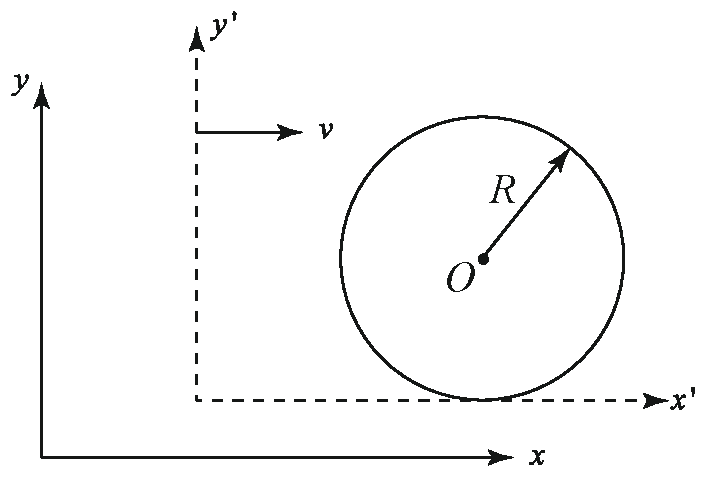
\includegraphics[width = 0.3\textwidth]{images/relativity-8.pdf} 
\end{flushright}
\tagged{student}{\vspace*{1cm}}
\begin{taggedblock}{teacher}
\noindent
解析:根据收缩效应可知圆变成了椭圆,长轴垂直于运动方向,依然为$R$,短轴沿运动方向,变成了$\sqrt{1-\frac{v^2}{c^2}}R$。
\end{taggedblock}
\end{example}
%%%%%%%%%%%%%%%%%%%%%%



%%%%%%%%%%%%%%%%%
\begin{example}
一根长度为$l_0$的棒,静止地平放在坐标系的$x'y'$平面上,与$x$轴所成的角度为$\theta_0$,在实验室坐标系$xy$中,棒以速度$v$沿$x$轴正方向运动,求在实验室坐标系中棒的长度$l$和它与$x$轴的夹角$\theta$。
\begin{flushright}
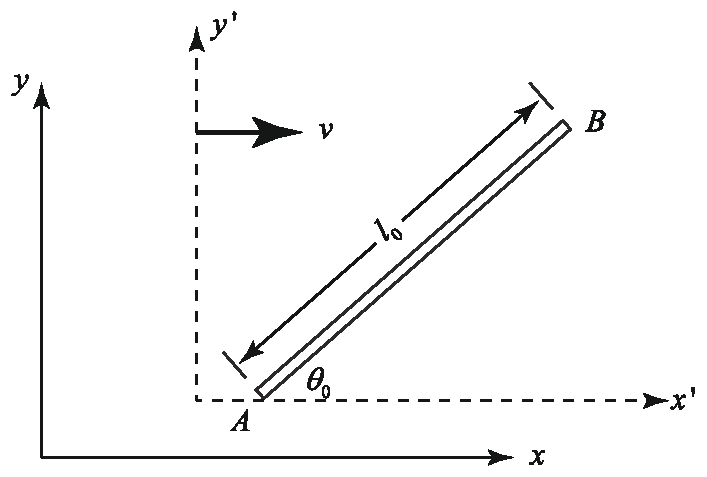
\includegraphics[width = 0.4\textwidth]{images/relativity-7.pdf} 
\end{flushright}

\tagged{student}{\vspace*{2cm}}
\begin{taggedblock}{teacher}
\noindent
解析:由于长度收缩,运动方向上长度变短,垂直于运动方向长度不变,这样
\[
l' = \sqrt{1- \frac{v^2}{c^2}\cos\theta_0},\qquad \tan\theta' \frac{1}{\sqrt{1-\frac{v^2}{c^2}}}\tan\theta
\]
\end{taggedblock}
\end{example}
%%%%%%%%%%%%%%%%%%%%%%

\subsection{相对论的速度叠加}
在经典力学的速度叠加原理我们已经学过了,考虑一列以速度$v$匀速行驶的列车,车头有一个光源,按照经典力学的速度叠加原理相对地面静止的观察者看到的光速度应当是$v+c$,而在前面我们已经看到在相对论当中超光速运动是不可能的。

相对论的速度叠加不满足平行四边形法则,考虑一个相对于参考系$S$做匀速运动的物体,它的速度分量分别为$(u_x,u_y,u_z)$,那么在$S$系当中它的运动方程为
\begin{equation}
x=u_xt,\qquad y=u_yt,\qquad z=u_zt
\end{equation}
在相对于$S$匀速运动的$S'$系所看到的运动由洛伦兹变换相联系:
\begin{eqnarray*}
x'&=&\frac{x-vt}{\sqrt{1-\frac{v^2}{c^2}}}=\frac{u_xt-vt}{\sqrt{1-\frac{v^2}{c^2}}}\\
y'&=&y=u_yt\\
z'&=&z=u_zt\\
t'&=&\frac{t-\frac{v}{c^2}x}{\sqrt{1-\frac{v^2}{c^2}}}=\frac{t-\frac{v}{c^2}u_xt}{\sqrt{1-\frac{v^2}{c^2}}}\\
\end{eqnarray*}
这样我们就可以很容易地得到$S'$系中所看到的运动速度$(u_x',u_y',u_z')$与相对于$S$的速度之间的联系
\begin{eqnarray*}
u_x'=\frac{x'}{t'}&=&\frac{u_x-v}{1-\frac{vu_x}{c^2}}\\
u_y'=\frac{y'}{t'}&=&\frac{u_y\sqrt{1-\frac{v^2}{c^2}}}{1-\frac{vu_x}{c^2}}\\
u_z'=\frac{z'}{t'}&=&\frac{u_z\sqrt{1-\frac{v^2}{c^2}}}{1-\frac{vu_x}{c^2}}
\end{eqnarray*}
很明显可以看到,平行四边形法则不再成立,并且沿着和垂直相对运动方向的速度变换的方式也有不同。
根据上面给出的速度变换公式,可以很容易地证明相对一个参考系的运动速度为光速的物体相对于另一个参考系的运动速度同样也为光速!


%%%%%%%%%%%%%%%%%
\begin{example}
证明以上结论,当一个物理对象相对于参考$S$的运动速度为$c$时,它相对于任意相对$S$匀速直线运动参考系中的速度也是$c$。
\tagged{student}{\vspace*{4cm}}
\begin{taggedblock}{teacher}
\noindent
解析:令相对于$S$的速度$u_x = c\cos\theta, u_y = c\sin\theta$,将它们代入速度变换公式可得
\[
u_x' = \frac{c\cos\theta-v}{1- \frac{v}{c}\cos\theta},\qquad u_y' = \frac{c\sin\theta\sqrt{1- \frac{v^2}{c^2}}}{1- \frac{v}{c}\cos\theta},
\]
它们的平方和
\[
u_x'^2+u_y'^2 = \frac{c^2\cos^2\theta-2vc\cos\theta+v^2+c^2\sin^2\theta -v^2\sin^2\theta}{(1-\frac{v}{c}\cos\theta)^2} = c^2
\]
\end{taggedblock}
\end{example}
%%%%%%%%%%%%%%%%%%%%%%


%%%%%%%%%%%%%%%%%
\begin{example}

有两个以速度$v_1$、$v_2$同向运动的物体$A$和$B$,求证当它们的速度远小于光速$v_{1,2}\ll c$时,$B$相对于$A$的速度满足经典的速度合成法则
\[
v_{B\rightarrow A} = v_2-v_1.
\]
\tagged{student}{\vspace*{4cm}}
\begin{taggedblock}{teacher}
\noindent
解析:关键在于理解相对论公式的含义,而不是去死记公式,这一点很重要。
\end{taggedblock}
\end{example}
%%%%%%%%%%%%%%%%%%%%%%



\subsection{多普勒效应和光行差}
假设有一个光源位于参考系$S$的原点处,它沿着与$x$轴夹角为$\theta$的方向发射了束频率为$\nu$的光。
在与$S$以速度$v$沿着$x$轴做匀速运动的参考系$S'$的观察者看来,这束光的频率和方向都会发生变化。
下面我们来仔细地看一下这个现象。

假设该光束被限制在$(x-y)$平面上,这样它的相位可由
\begin{equation}\label{eqn: S系中的相位}
\omega\left(t-\frac{\cos\theta x+\sin\theta y}{c}\right)
\end{equation}
同样一束光在$S'$看来假设它的相位是由
\begin{equation}
\omega'\left(t'-\frac{\cos\theta' x'+\sin\theta' y'}{c}\right)
\end{equation}
来给出。
可以将光波相位(标量)取不同值看成一个事件,不同参考系中对其没有异议。
例如光波中电场强度出现极大值时所有的观察者看到的电场强度都是最大值\footnote{用现代的语言来讲,相位是一个洛伦兹标量,所有的观察者看到的值是一样的。}。
这样$s'$系中的相位可由洛伦兹变换的逆变换代入相位\ref{eqn: S系中的相位}当中得到:
\begin{equation}
\sin\omega\left(\frac{t'+\frac{v}{c^2}x'}{\sqrt{1-\frac{v^2}{c^2}}}-\frac{\cos\theta \frac{x'+vt'}{\sqrt{1-\frac{v^2}{c^2}}}+\sin\theta y}{c}\right)
\end{equation}
并与$S'$中的相位相比,我们需要$(x',y',t')$的系数在两式当中完全相同,这样就可以得到
\begin{eqnarray}
\omega'&=&\frac{1-\frac{v}{c}\cos\theta}{\sqrt{1-\frac{v^2}{c^2}}}\omega\\
\cos\theta'&=&\frac{\cos\theta-\frac{v}{c}}{1-\frac{v}{c}\cos\theta}
\end{eqnarray}
从中可以看出相对运动的观察者看到的光的频率和传播方向都有了变化。

频率的变化不是别的,正是相对论中的{\heiti 多普勒效应}(Doppler effect):当光源和观察者有相对运动时光的频率会发生变化,并且当光源向着观察者运动时$(v<0)$频率将增加,反之光源远离观察者时频率会变小。
细心的同学应该已经看出相对论中的多普勒效应是经典力学的多普勒效应与时间膨胀效应的叠加。
光线传播方向的变化被称做{\heiti 光行差}(light aberration),上式得到的光行差的结果与以与$x$轴正方向夹角为$\theta$以光速度运动的物体在$S'$系当中看到的速度方向一致,可以自行证明这一点。

%%%%%%%%%%%%%%%%%%%%%%%%%%%%%%%%%%
\begin{example}
已知无限远处一个恒星发出的光到达太阳系时与地球运行方向夹角为$\theta$,地球此时的速度为$v_0$,求地球上看此光的夹角。
\begin{flushright}
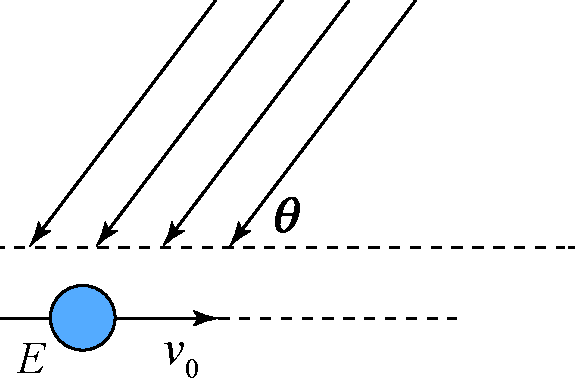
\includegraphics[width=0.4\textwidth]{images/relativity-1.pdf}
\end{flushright}
\tagged{student}{\vspace*{1cm}}
\begin{taggedblock}{teacher}
\noindent

解析:\[\cos \theta^\prime = \frac{\cos \theta +\frac{v_0}{c}}{1+\frac{v_0}{c}\cos\theta}\]
\end{taggedblock}
\end{example}
%%%%%%%%%%%%%%%%%%%%%%%%%%


%%%%%%%%%%%%%%%%%%%%%%%%%%%%%%%%%%
\begin{example}
当一艘飞船静止时前部探照灯发出的光束与飞船轴线的夹角为$\theta$,如图所示。
当飞船以速度$v_0$飞得时求处于静止的观察者所看到的光束的夹角。
\begin{flushright}
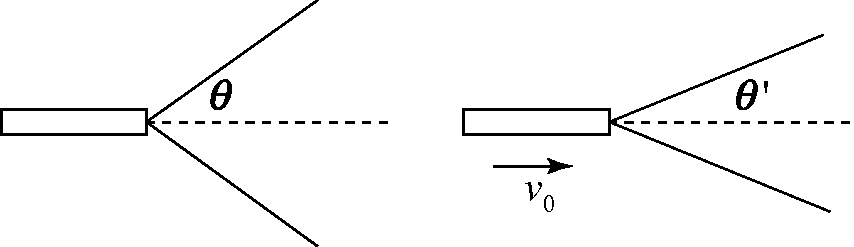
\includegraphics[width=0.5\textwidth]{images/relativity-2.pdf}
\end{flushright}
\tagged{student}{\vspace*{4cm}}
\begin{taggedblock}{teacher}
\noindent

解析:\[\cos \theta^\prime = \frac{\cos \theta +\frac{v_0}{c}}{1+\frac{v_0}{c}\cos\theta}\]
\end{taggedblock}
\end{example}
%%%%%%%%%%%%%%%%%%%%%%%%%%



\section{相对论的动力学}
在相对论中我们之前学过的运动定律、动量动能定理等在不同的参考系当中应当具有相同的形式。
需要指出的是当运动速度极快(相对论性)的质点满足的运动定律并不一定是牛顿第二定律
\begin{equation}\label{eqn: 相对论,粒子的运动方程}
\vec{f}=m\frac{d\vec{v}}{dt}
\end{equation}
因为这样的方程并不满足相对性原理。
但是如果质点的运动速度与光速相比极小,上式还是成立的,因为它已经被实验所证实。
相对论下牛顿第一定律与牛顿第三定律的正确性仍然是毋庸置疑的。仔细地思考,我们可以发现牛顿第二定律和牛顿第三定律的结合实际上导致了动量的守恒,而牛顿第二定律不过是把动量的改变率定义为力,它代表相互作用的强度。所以我们仍然猜想相对论下物理过程的动量守恒\footnote{为什么动量一定要守恒呢?动量守恒实际上是时空在平移操作下的不变性导致的。这样的对称性与守恒率的关系还有很多,有兴趣的同学可以去了解更多内容。}。


考虑在一个给定的参考系$S'$中有两个质量同为$m$的质点以相等并且远小于光速的速度$u'$相向运动,并在坐标系的原点处发生完全非弹性碰撞并合成一个质点。
根据对称性可知无论在相对论当中动量被表达成什么形式,两个质点的动量总是大小相等方向相反的,完全非弹性碰撞以后相对于$S'$必然静止在原点处。
和前面一样假设$S'$相对于$S$以速度$v$沿着$x$轴匀速直线运动。
在$S$看来,两个质点的运动速度分别为
\begin{equation}
u_{1}=\frac{v-u}{1-\frac{vu}{c^2}},\qquad u_{2}=-\frac{v+u}{1+\frac{vu}{c^2}}
\end{equation}
在发生完全非弹碰撞以后,根据在$S'$系中的结果可知必然会形成一个新的质点以速度$v$沿着$x$轴正向运动。
但如果此时你依然认为动量保持在经典力学中的形式$p=mv$,以及在完全非弹性碰撞过程中动量守恒,那么简单的计算将表明在$S$系中得到不正确的结果。

为了使牛顿第二定律在不同的参考系中成立,以及得到碰撞过程中正确的结果,那么必须重新定义运动物体的动量为
\begin{equation}
\vec{p} = \frac{m\vec{v}}{\sqrt{1-\frac{v^2}{c^2}}}
\end{equation}
力,作为相互作用的量度,仍然定义为动量对时间的导数:
\begin{equation}\label{eqn: Newton.II}
\vec{F}=\frac{d}{dt}\vec{p} = \frac{d}{dt}\left[\frac{m\vec{v}}{\sqrt{1-\frac{v^2}{c^2}}}\right].
\end{equation}
这就是修正了的相对论中的牛顿第二定律。在碰撞过程中,动量守恒的要求便是牛顿第三定律的成立(一质点动量的增加等于另一质点动量的减小)。

值得指出,如果坚持认为动量是质量和速度的乘积的话,从上式可以看出运动物体的质量与速度有关,随着速度的增加质量也会增加,当速度接近光速时质量变为无限大,相同的力对它产生的加速度越来越小,直至变为零。
这就从动力学的角度解释了为什么自然界任何物体的速度都不可能超过光速。这样的质量被称为质点的{\heiti 动质量}或{\heiti 相对论性质量}(relativistic mass)
从上式可以很容易地看出高速运动质点的动质量$m_v$与其静止质量$m$的关系为
\begin{equation}
m_v = \frac{m_0}{\sqrt{1- \frac{v^2}{c^2}}}.
\end{equation}
而原来的质量则被称为{\heiti 不变质量}(invariant mass)或{\heiti 静质量}(rest mass)以示区别。正如其名称所暗示的,质点速度为零时其动质量最低,大小即为其静质量。而所谓不变质量$m$,说明$m$是质点的基本属性,它不随着参考系的变化而变化,基本粒子的不变质量即是物理学基本常数。

不但动量,能量在相对论中也必须重新定义才能够满足相对性原理。
如果在相对论中当我们依然将力沿着位移方向分量的积分依然称为功的话,对于一个由静止出发在不变的力$F$作用下加速度运动的质点来说,力所做的功
\begin{equation}
\int F dx = \int_0^t F vdt
\end{equation}
其中$t$为由静止开始将质点加速到速度$v$所需要的时间,将\ref{eqn: Newton.II}代入上式可得
\begin{equation}
\int_0^t F vdt=\int_0^v v \cdot \frac{d}{dt}(\frac{mv}{\sqrt{1-\frac{v^2}{c^2}}})dt=\int_0^v \frac{mv}{(1-\frac{v^2}{c^2})^{3/2}}\frac{dv}{dt}dt=\frac{mc^2}{\sqrt{1-\frac{v^2}{c^2}}}-mc^2
\end{equation}
如果我们坚持动能定理(即能量守恒)的话,上式求出的量就被称做物体的动能$E_k$。

对于远低于光速度的速度$v$,动能可以近似表达为
\begin{equation}
c^2\left(1-\frac{v^2}{c^2}\right)^{-\frac{1}{2}}-mc^2\simeq mc^2\left(1+\frac{1}{2}\frac{v^2}{c^2}\right)-mc^2=\frac{1}{2}mv^2
\end{equation}
可见与牛顿力学当中的动能表达式一致,但是当速度与光速相比不是那么小的话,就会与经典力学有明显的偏离,这时我们就必须使用
\begin{equation}\label{eqn: 相对论,相对论性的动能}
E_k=\frac{mc^2}{\sqrt{1-\frac{v^2}{c^2}}}-mc^2
\end{equation}
来表示运动物体的动能。
当得到这个结果以后爱因斯坦做了一个极其大胆的假设,在他眼里式\ref{eqn: 相对论,相对论性的动能}并不是简单地看做运动物体的动能,而是一个物体在运动与静止状态的能量差。
这样物体的能量与运动速度的关系就变成了
\begin{equation}\label{eqn: relativity-e=mcsqre/sqrt}
E=\frac{mc^2}{\sqrt{1-\frac{v^2}{c^2}}}
\end{equation}
基于这个假设,不但运动的物体具有能量,一个静止的物体同样具有能量
\begin{equation}
E_0=mc^2
\end{equation}
这就是著名的爱因斯坦的{\heiti 质能方程}(mass-energy equivalence),它表明即使一个处于静止状态的物体也具有它的质量与光速平方乘积的能量,称为{\heiti 静能量}(rest energy)。
这样,运动的质点的能量即为其静能量$E_0$与其动能$E_k$的和:
\[E=E_0+E_k\]
质能方程的一个直接推论就是如果一个物理过程前后物体的静质量有所变化时,假设静质量变化为$\Delta m$,那么将会释放出
\begin{equation}
\Delta E = \Delta m c^2
\end{equation}
的动能,因为总能量守恒。
这一事实被随后的实验所证实,这是相对论最为光辉的成就,它为人类寻找新的能源打开了一道门。

通常来说宏观物体的运动速度与光速相比几乎可以忽略不计,因为它们的质量很大,很难将它们加速到接近于光速,所以利用经典物理学来描写它们的运动很成功。
但是对于那些质量很小的对象,例如原子或电子时,由于它们的小质量,只需要不大的能量就可以获得极大的速度,这时就必须使用相对论来描写它们的运动和相互作用\footnote{更加准确的说,小的尺寸决定了其考虑量子力学的必要性,而在量子力学的框架下时空尺度越小,对应的特征能量越大。}。
微观粒子的碰撞会引起速度很大的变化,但在相互作用过程中动量和能量的守恒是必须成立的,但是需要注意的是这时不能够使用经典力学中动量和能量的定义,而是换成相对论性的动量和能量。
另外要特别强调的是一个静止的物体在经典力学中是没有动力学意义下的能量的(除了外势能),但在相对论当中则具有很大的能量,也就是它们的质能$mc^2$,其中$m$为它的静止质量。

%%%%%%%%%%%%%%%%%%%%%%%%%%%%%%%%%%
\begin{example}
太阳的辐射功率约为$P = 3.828\pow{26}\unit{W}$,根据质能方程估算太阳一年当中质量的变化量。
已知太阳的质量约为$M_S\sim 1.99\pow{30}\unit{kg}$,估算一亿年太阳质量的相对变化量。
\tagged{student}{\vspace*{4cm}}
\begin{taggedblock}{teacher}
\noindent

解析:简单的计算可知太阳一年之中质量的损失约为
\[
\Delta M \simeq \frac{P}{c^2}\cdot 60\cdot 60\cdot 24\cdot 365 = 1.3\pow{17}\unit{kg}
\]
这样1亿年中太阳辐射造成的质量损失与总质量的比值
\[
\frac{1.3\pow{17}\times 10^{8}}{M_S}\simeq 6.7\pow{-6}
\]
可以看出虽然质量损失巨大,但与太阳质量比起来其实依然微不足道。
\end{taggedblock}
\end{example}
%%%%%%%%%%%%%%%%%%%%%%%%%%


%%%%%%%%%%%%%%%%%%%%%%%%%%%%%%%%%%
\begin{example}
实验中观察到如下的原子核反应:稳定的$^{235}{\rm U}$在吸收了一个动能可以忽略不计的中子之后发生裂变:
\[
^{235}{\rm U}+^1n\rightarrow ^{94}{\rm Zr}+^{140}{\rm Ce}+2^1n+\Delta E.
\]
试估计裂变释放能量$\Delta E$的大小,用$\unit{MeV}$来表示结果。
已知$m(^{235}{\rm U}) = 235.044\unit{u}$; $m(^{94}{\rm Zr}) = 93.9063\unit{u}$;$m(^{140}{\rm Ce}) = 139.905\unit{u}$;$m(^{1}n) = 1.00867\unit{u}$;其中$u$为原子单位$1u=931.502\unit{Mev/c^2}$。
忽略反应过程中的电荷不守恒问题。
\tagged{student}{\vspace*{4cm}}
\begin{taggedblock}{teacher}
\noindent

解析:反应前后的质量变化
\[
\Delta m = \left[m(^{235}{\rm U})+m(n)\right]-\left[m({\rm Ze})+m({\rm Ce})+2m(n)\right] = 0.22403~u
\]
这样根据质能方程
\[
\Delta E = \Delta m\cdot c^2 =  0.22403~u \times 931.502 ~\rm{MeV}~c^{-2} c^2 = 208.684~\rm{MeV}
\]
\end{taggedblock}
\end{example}
%%%%%%%%%%%%%%%%%%%%%%%%%%


%%%%%%%%%%%%%%%%%
\begin{example}
求一个静止质量为$m_0$的质点在恒力$F$作用下位置随时间的关系$x(t)$,已知$t=0$时它位于坐标系原点处($x(0) = 0$)且速度为0。
\tagged{student}{\vspace*{4cm}}
\begin{taggedblock}{teacher}
\noindent

解析:利用相对论性运动方程,在恒力$F$作用下有
\[Ft = \frac{mv}{\sqrt{1-\frac{v^2}{c^2}}},\]
从上式中可解出$v(t)$:
\[
v(t) = \frac{dx(t)}{dt} = \frac{Ft}{\sqrt{m^2+\frac{F^2t^2}{c^2}}},
\]
积分可得:
\[
x(t) = \int_0^t\frac{F\tau}{\sqrt{m^2+\frac{F^2\tau^2}{c^2}}}d\tau = \frac{c^2}{F}\left[\sqrt{m^2+\frac{F^2t^2}{c^2}}-m\right] = \frac{mc^2}{F}\left[\sqrt{1+\frac{F^2t^2}{m^2c^2}}-1\right]
\]
\end{taggedblock}
\end{example}
%%%%%%%%%%%%%%%%%%%%%%

%%%%%%%%%%%%%%%%%
\begin{example}
一个静止质量为$m_0$的粒子在一惯性参考系中做直线运动,其坐标与时间的关系为
\[
x(t) = \sqrt{b^2+c^2t^2}-b,
\]
求粒子所受外力随时间的关系。
\tagged{student}{\vspace*{4cm}}
\begin{taggedblock}{teacher}
\noindent

解析:直接和上式类比即可,也可以根据定义计算。
\end{taggedblock}
\end{example}
%%%%%%%%%%%%%%%%%%%%%%


%%%%%%%%%%%%%%%%%%%%%%%%%%%%%%%%%%
\begin{example}
求证一个静止质量为$m_0$的高速运动质点的能量$E$和动量$p$之间满足
\[
E^2 = p^2c^2+m^2c^4
\]
\tagged{student}{\vspace*{4cm}}
\begin{taggedblock}{teacher}
\noindent

解析:简单代入以后即可发现,注意本题的解给出了动量、能量之间的一个关系。
另外在开平方的时候有一个正负号问题,它能够引出丰富的物理内容。
\end{taggedblock}
\end{example}
%%%%%%%%%%%%%%%%%%%%%%%%%%


%%%%%%%%%%%%%%%%%
\begin{example}
实验观测表明,带电介子$\pi^\pm$主要衰变为一个$\mu^\pm$轻子和一个$\mu$子型中微子$\nu_\mu$:
\[
\pi^+\rightarrow\mu^++\nu_\mu.
\]
已知$m_\pi = 139.6\unit{MeV/c^2}$,$m_\mu = 105.7\unit{MeV/c^2}$,忽略中微子的质量,求静止的$\pi$介子衰变产物中$\mu$轻子的运动速度。
\tagged{student}{\vspace*{4cm}}
\begin{taggedblock}{teacher}
\noindent

解析:由动量守恒:
\[p_\nu = p_\mu\]
轻子$\mu$的能量与中微子$\nu$的能量分别为:
\[E_\mu=\sqrt{p_\mu^2+(m_\mu c^2)^2}\]
\[E_\nu = p_\nu c=p_\mu c\]
能量守恒:
\[E_\mu + E_\nu = m_\pi c^2\]
解得:
\[p_\mu=29.8\unit{MeV/c^2}\, , \, E_\mu=109.8\unit{MeV/c^2}\, , \, v_\mu=\frac{p_\mu c^2}{E_\mu}=0.271c\]
\end{taggedblock}
\end{example}
%%%%%%%%%%%%%%%%%%%%%% 


%%%%%%%%%%%%%%%%%
\begin{example}

在高能物理中实验表明,在实验室参考系中一个运动的质子与一个静止的质子相碰后可能再产生一个质子和一个反质子,即总共存在三个质子和一个反质子。
试求发生这一情况时,碰前那个运动质子的能量(相对实验室参考系)的最小值(即阈值)是多少。
已知质子和反质子的静止质量均为$m_0 = 1.67\pow{-27}\unit{kg}$,不考虑粒子之间的电相互作用。
\tagged{student}{\vspace*{4cm}}
\begin{taggedblock}{teacher}
\noindent

解析:\[E_{th}=7m_0 c^2=6.56\unit{GeV}\]
\end{taggedblock}
\end{example}
%%%%%%%%%%%%%%%%%%%%%%



%%%%%%%%%%%%%%%%%
\begin{example}

证明相对论中一个静止质量为$m$质点在两个相对运动参考系中的动量和能量之间有如下的变换关系:
\begin{eqnarray*}
p_x' &=& \frac{p_x-\frac{v}{c^2}E}{\sqrt{1-\frac{v^2}{c^2}}}\\
p_y' &=& p_y\\
p_z' &=& p_z\\
E' & = & \frac{E-vp_x}{\sqrt{1-\frac{v^2}{c^2}}}
\end{eqnarray*}
\tagged{student}{\vspace*{4cm}}
\begin{taggedblock}{teacher}
\noindent

解析:略
\end{taggedblock}
\end{example}
%%%%%%%%%%%%%%%%%%%%%%





%%%%%%%%%%%%%%%%%
\begin{example}

【思考】试求两个相对运动参考系之间电荷密度和电流密度之间的变换关系。
\tagged{student}{\vspace*{4cm}}
\begin{taggedblock}{teacher}
\noindent

解析:
\begin{eqnarray*}
j_x' &=& \frac{j_x-v \rho}{\sqrt{1-\frac{v^2}{c^2}}}\\
j_y' &=& j_y\\
j_z' &=& j_z\\
\rho' & = & \frac{\rho-\frac{v}{c^2}j_x}{\sqrt{1-\frac{v^2}{c^2}}}
\end{eqnarray*}
\end{taggedblock}
\end{example}
%%%%%%%%%%%%%%%%%%%%%%




\section{不同参考系中的电磁场}
根据电磁学和相对性原理,一个相对于运动参考系$S'$系静止的带电粒子将会产生一个静电场。
但是相对于地面来说它将是一个运动着的带电粒子,除了电场以外它还会像一个电流一样产生磁场。
它所产生的电场和磁场可以对一个运动的带电粒子应用电磁学定律而得到。
但是因为两个参考系中的观测者其实都在描写一个带电物体的电磁学效应,只是观察方式不同而已。
和时空坐标一样,不同的观测者所看到的电磁场也是有联系的。

但是等等,我们需要先明确一下电磁场大小的定义。其实很简单,即使在相对论的情况下,试探电荷静止时受到的力与电荷的比定义了电场强度,而运动时其受到的额外的力与其运动速度的关系则定义了磁感应强度。也就是说洛伦兹力公式仍然成立:
\[\vec{F}=q(\vec{E}+\vec{v}\times\vec{B})\]

假设在$S$系当中在时间$t$,坐标$(x,y,z)$处存在一个电场,它的三个分量分别为$(E_x,E_y,E_z)$,与此同时在相同的点上也有一个磁场,磁场的分量则用$(B_x,B_y,B_z)$来给出。
那么在$S'$系当中,上面所述的时空点由洛伦兹变换\ref{eqn: x的Lorentz变换}-\ref{eqn: t的Lorentz变换}所给出,与此同时在$(x',y',z',t')$点处也会看到一个电磁场,该电磁场的场强并不与$S$系当中所观测到的场强相等,而是由变换
\begin{eqnarray}\label{eqn: 电磁场的Lorentz变换}
&E_x'=E_x \qquad &B_x'=B_x\\
&E_y'=\frac{E_y-vB_z}{\sqrt{1-\frac{v^2}{c^2}}}\qquad &B_y'=\frac{B_y+\frac{v}{c^2}E_z}{\sqrt{1-\frac{v^2}{c^2}}}\\
&E_z'=\frac{E_z+vB_y}{\sqrt{1-\frac{v^2}{c^2}}}\qquad &B_z'=\frac{B_z-\frac{v}{c^2}E_z}{\sqrt{1-\frac{v^2}{c^2}}}
\end{eqnarray}
从中可以看出,电磁场沿着运动方向的分量不会发生变化,但垂直于运动方向会有变化。
一个值得指出的事实是电场和磁场在相对论中是一个相对的概念。可以这样思考:所谓电场和磁场的二分是根据电磁场物质对电荷的作用力与电荷运动状态的关系而引入的数学上的划分。参考系变了,原来静止的粒子将要运动,原来运动的粒子可能静止。粒子受到的力也将参与洛伦兹变换。所以电磁场中电场与磁场分量的值可能发生改变。一个物理体系在一个参考系中如果只有电场,在另一个参考系中测量可能同时存在电场和磁场。

%%%%%%%%%%%%%%%%%%%%%%%%%%%%%%%%%%
\begin{example}
有一个充好电的平行板电容器,极板面积为$S$,相距$L$,所带电量是$Q$。
求一个以速度$v$从电空器中间穿过电子看来两板之间的电势差以及穿过前后电子能量的变化量。
\tagged{student}{\vspace*{4cm}}
\begin{taggedblock}{teacher}
\noindent
解析:由于动尺缩短所以电子看来两板之间的距离
\[
L' = \sqrt{1- \frac{v^2}{c^2}}L,
\]
而又因为电场在电子运动方向的分量不同参考系中保持不变,所以电子在电容两板之间运动时电场力作用距离变小,两板之间的电势差
\[
U' = \frac{QL'}{ \varepsilon_0 S} = \sqrt{1- \frac{v^2}{c^2}}U,
\]
其中$U$是静止系看起来两板之间的电势差。能量变化量:
\[\Delta E=QU'\]
\end{taggedblock}
\end{example}
%%%%%%%%%%%%%%%%%%%%%%%%%%


%%%%%%%%%%%%%%%%%
\begin{example}

考虑通电导线的一个简单模型:一根无限长直线上有均匀分布的正负电荷,每个电荷带电量为$\pm q$,相邻两个电荷之间距离为$l$,其中负电荷静止,正电荷以速度$v$向右运动。
回答下面几个问题:

1. 此时导线中的电流是多少;

2. 与导线相距$d$的一点$P$处的磁感应强度为多少;

3. 如果P点处有一个带正电的粒子$Q$以相同的速度$v$向右运动,求它受到的洛伦兹力大小和方向;

4. 在一个以速度$v$向右运动的参考系中,导线中的电流是多少?导线带电吗?如果不带电请说明理由,如果带电请算出电荷线密度;

5. 在两个参考系中分别描写带电粒子P的运动和受力。

\tagged{student}{\vspace*{4cm}}
\begin{taggedblock}{teacher}
\noindent
解析:1. 
\[\lambda = \frac{q}{l}\]
\[I=\lambda v=\frac{qv}{l}\]
2. \[B=\frac{\mu_0 I}{2\pi d}=\frac{\mu_0 qv}{2\pi dl}\]
3. 方向指向导线,大小:
\[F=QvB=\frac{\mu_0 Qqv^2}{2\pi dl}\]
4. \[\lambda_+'=\lambda \cdot \sqrt{1-\frac{v^2}{c^2}}\; , \; \lambda_-'=-\lambda\cdot \frac{1}{\sqrt{1-\frac{v^2}{c^2}}}\]
\[\lambda'=\lambda_-'+\lambda_+'=-\frac{\frac{v^2}{c^2}}{\sqrt{1-\frac{v^2}{c^2}}}\cdot \frac{q}{l}\]
\[I'=\lambda_-'\cdot(-v)=\frac{1}{\sqrt{1-\frac{v^2}{c^2}}}\cdot\frac{qv}{l}\]
5. 以指向导线为正,由于$Q$静止,受力仅为电场力:
\[F'=F_E'=-Q\cdot \frac{\lambda'}{2\pi\varepsilon_0 d}=\frac{\mu_0 Qqv^2}{2\pi dl\sqrt{1-\frac{v^2}{c^2}}}\]
\end{taggedblock}
\end{example}
%%%%%%%%%%%%%%%%%%%%%%




%%%%%%%%%%%%%%%%%
\begin{example}
【课后思考题】当空间中的电荷密度、电流密度随的变化由已知函数$\rho,j_x,j_y,j_z$
所给出时,在一惯性参考系$S$中电磁场变化所满足的麦克斯韦方程组有微分形式:
\begin{eqnarray*}
\frac{\partial E_x}{\partial x}+\frac{\partial E_y}{\partial y}+\frac{\partial E_z}{\partial z} = \frac{1}{\varepsilon_0}\rho\\ 
\frac{\partial B_x}{\partial x}+\frac{\partial B_y}{\partial y}+\frac{\partial B_z}{\partial z} = 0
\end{eqnarray*}
\begin{eqnarray*}
\frac{\partial E_z}{\partial y}-\frac{\partial E_y}{\partial z} = -\frac{\partial B_x}{\partial t}\qquad  \frac{\partial B_z}{\partial y}-\frac{\partial B_y}{\partial z} = \mu_0 j_x+\mu_0\varepsilon_0\frac{\partial E_x}{\partial t}\\
\frac{\partial E_x}{\partial z}-\frac{\partial E_z}{\partial x} = -\frac{\partial B_y}{\partial t}\qquad  \frac{\partial B_x}{\partial z}-\frac{\partial B_z}{\partial x} = \mu_0 j_y+\mu_0\varepsilon_0\frac{\partial E_y}{\partial t}\\
\frac{\partial E_y}{\partial x}-\frac{\partial E_y}{\partial x} = -\frac{\partial B_z}{\partial t}\qquad \frac{\partial B_y}{\partial x}-\frac{\partial B_x}{\partial y} = \mu_0 j_z+\mu_0\varepsilon_0\frac{\partial E_z}{\partial t}
\end{eqnarray*}
以上各个物理量的自变量均为$(x,y,z,t)$,当另一个参考系$S'$以速度$v$沿着$S$的$x$轴方向匀速运动时,根据相对性原理相对于它麦克斯韦方程组也需要保持相同的形式。请根据上一讲最后一题给出的电荷,电流洛伦兹变换公式和本节的场的变换公式验证其协变性。


\tagged{student}{\vspace*{0cm}}
\begin{taggedblock}{teacher}
\noindent
解析:略
\end{taggedblock}
\end{example}
%%%%%%%%%%%%%%%%%%%%%%




